\documentclass[12pt]{article}
\usepackage[english]{babel}
\usepackage{amsmath,amsthm}
\usepackage{graphicx}
\usepackage{caption}
\usepackage{subcaption}
\usepackage{graphicx}
\usepackage{amsfonts}
\usepackage{indentfirst}
\usepackage{lscape}
\usepackage[top=2.5cm,bottom=2.5cm,right=2.5cm,left=2.5cm]{geometry}
\usepackage{titlesec}
\setcounter{secnumdepth}{5}

% ----------------------------------------------------------------
\begin{document}

\section{Color Constrast Occurence}

Here we will see the different steps that we have to follow to compute the C$_2$O descriptor. There will be three main steps that we will have to study, The transformation through a perceptual space, the computation of the coocurence matrix and the computation of the signature vector.

\subsection{Transformation through a perceptual space}

First of all, we need to pass our image in the L$^*$a$^*$b$^*$ space to get directly a representation of our image in a space which split the luminance and the chromatic information.

For doing that, we first need to pass the image in the XYZ space and choose the correct standard illuminant A. 
\vspace{0.5cm}
$$A=\begin{pmatrix}
	X_r&X_g&X_b\\
	Y_r&Y_g&Y_b\\
    Z_r&Z_g&Z_b
\end{pmatrix}$$


That parameter depends on the characteristics of the device used to take the picture: it represents how the device interpret the real colors. In our case, there are many different devices that have been used to take the different pictures so we will have to make a choice. Some standard illuminant are defined by the illumination of the scene like D50 which corresponds to an "horizon light" contrary to D65 which correspond to a "noon light". Ideally, we will have to make the choice for each image but in front of the huge quantity of images, it will be need to make a choice.

\vspace{0.5cm}
\begin{equation}
\begin{pmatrix}X\\Y\\Z\end{pmatrix}=A*\begin{pmatrix}R\\G\\B\end{pmatrix}
\end{equation}

After doing this transformation, we can easily transform our image through the L$^*$a$^*$b$^*$ space.

\vspace{0.5cm}
\begin{equation}
L^*=  \left \{
   \begin{array}{l}
      116*(\frac{Y}{Y_0})^\frac{1}{3}-16~~~~si \frac{Y}{Y_0}>0.008856\\
   903.3*(\frac{Y}{Y_0})~~~~~~~~~~si \frac{Y}{Y_0}<0.008856\\
   \end{array}
   \right .
\end{equation}
\vspace{0.5cm}
\begin{equation}
a^*=500*\begin{bmatrix}f(\frac{X}{X_0})-f(\frac{Y}{Y_0})\end{bmatrix}
\end{equation}
\vspace{0.5cm}
\begin{equation}
b^*=300*\begin{bmatrix}f(\frac{Y}{Y_0})-f(\frac{Z}{Z_0})\end{bmatrix}
\end{equation}

\subsection{The coocurence matrix}

To obtain the concurrence matrix, we have to calculate an image of the difference of color. For that, the program will take the difference between each point of the image and the point which is at a distance following a $\Delta$ vector from it. This calculation will has the same result if we compute the difference between the original image and a copy of it translated following $\Delta$. (ColorDiff)

\begin{figure}[h]
    \center
    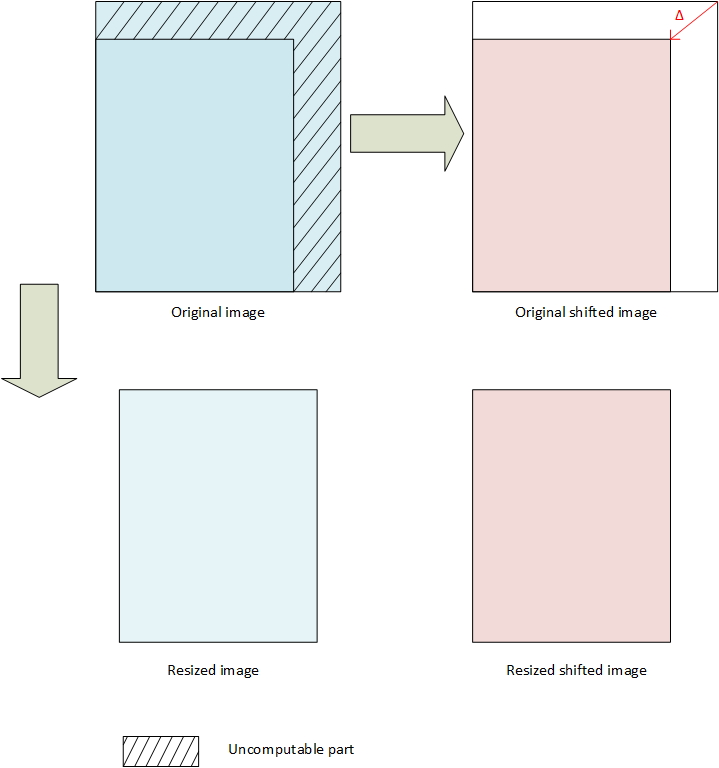
\includegraphics[scale=0.65]{ColorDiff.png}
    \caption{Color Difference illustration}\label{fig:Color Difference by image shifting illustration}
\end{figure}

To do that, the program will calculate the equivalent of the translation in horizontal and vertical pixel translation as show below .

\begin{figure}[h]
    \center
    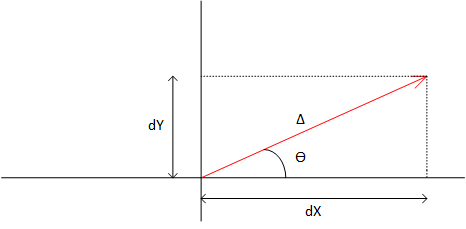
\includegraphics[scale=0.65]{illustrationVecteur.png}
    \caption{Vector to pixel distance}\label{fig:Vector to pixel distance}
\end{figure}

\begin{equation}
\begin{split}
&\sin\theta=dY/\|\Delta\| \\
&dY = \sin\theta * \|\Delta\| \\
&\cos\theta=dX/\|\Delta\| \\
&dX = \cos\theta * \|\Delta\| 
\end{split}
\end{equation}

The values of $\|\Delta\|$ and $\theta$ have to being choose in the aim of get an entire number of pixel.

This computation gives us the C$_2$O matrix which corresponds to the cloud of point described in the State of art. To validate this part, we have to compare our results with theory. It's known that the L$^*$a$^*$b$^*$ space has different component :
\begin{itemize}
\item L$^*$ which is an achromatic component
\item a$^*$ which express the opposition between the red and the green
\item b$^*$ which express the opposition between the blue and the yellow
\end{itemize}


\begin{figure}[h]
    \center
    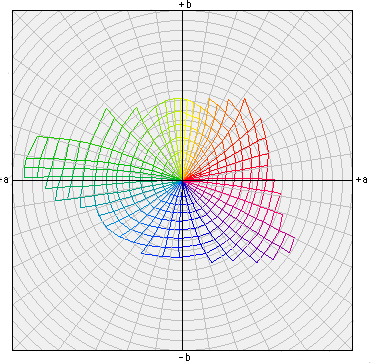
\includegraphics[scale=0.65]{BL_LAB.png}
    \caption{Lab space illustration}\label{fig:Lab space illustration}
\end{figure}

We define two test images :

So if we are testing our program on images like the two one shown below which are containing the two same colors opposed on the same component of the  L$^*$a$^*$b$^*$ space, the result on the difference must show that :

\begin{itemize}
\item For the first one which is in green and red, there will be two points spaced on the a$^*$ component but at constant levels on the L$^*$ and the b$^*$ component.
\item For the second one which is in blue and yellow, there will be two points spaced on the b$^*$ component but at constant levels on the L$^*$ and the a$^*$ component.
\end{itemize}


\begin{figure}[h]
        \centering
        \begin{subfigure}[b]{0.5\textwidth}
                \centering
                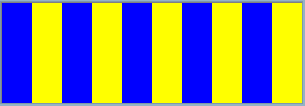
\includegraphics[height=70px]{TestIMG_BY.png}
        \end{subfigure}%
        \hfill
        \begin{subfigure}[b]{0.5\textwidth}
                \centering
                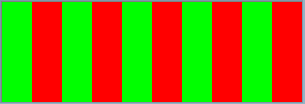
\includegraphics[height=70px]{TestIMG_RG.png}
        \end{subfigure}
        \caption{Test images}
        \label{fig:Test images}
\end{figure}

\begin{figure}[h]
        \centering
        \begin{subfigure}[b]{0.5\textwidth}
                \centering
                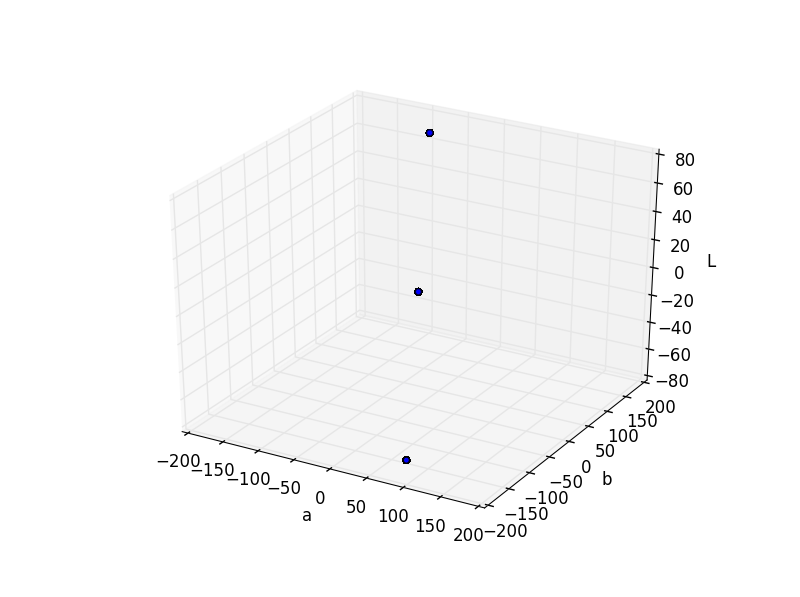
\includegraphics[height=228px]{CoocurenceMatrixForBlue_Yellow_grid.png}
        \end{subfigure}%
        \hfill
        \begin{subfigure}[b]{0.5\textwidth}
                \centering
                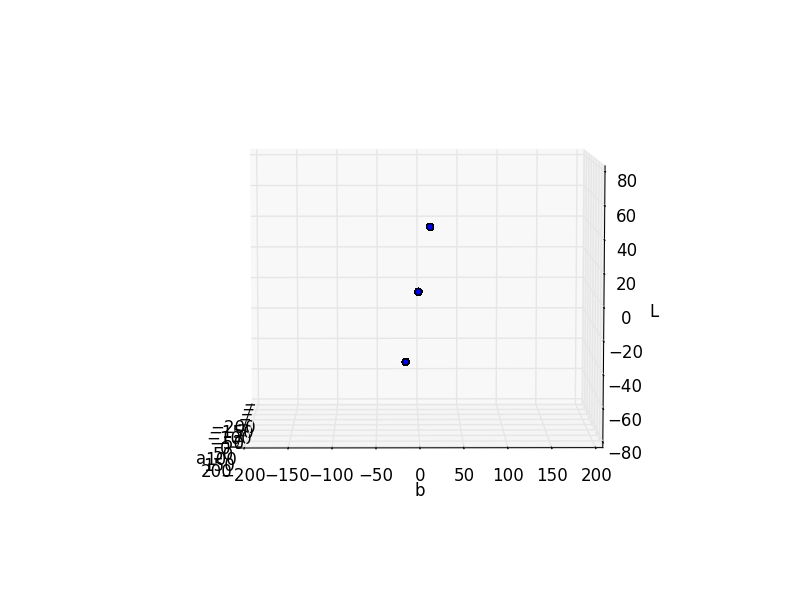
\includegraphics[height=228px]{CoocurenceMatrixForRed_Green_grid.png}
        \end{subfigure}
        \caption{Coorcurence matrix obtained from test images}
        \label{fig:Coorcurence matrix obtained from test images}
\end{figure}

With this step validate by the theory, we will have to test with more colors to verify that we obtain the right number of points on the coocurence matrix for the corresponding number of colors. (Test to add once the will be done (Appendix ?))


\subsection{The signature computing}

After doing that, we have to compute the spherical quantization of the probability matrix. For that, we have to transform our difference image for Carthesian coordinates to Spheric coordinates (from these one, the spherical quantization will be easier to compute). So we consider our Lab space like a 3 dimensional repository and for each points, it's calculate the norm of the vector formed by the distance between it and the point (0,0,0), the orientation $\alpha$ formed by the angle between the vector and the a plan and finally the orientation $\beta$ formed by the angle between the vector and the b plan.


\begin{figure}[h]
    \center
    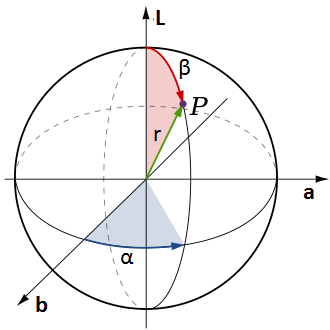
\includegraphics[scale=0.60]{Spherical_Coordinates.png}
    \caption{Spherical coordinates}\label{fig:Spherical coordinates}
\end{figure}


So for each pixel we obtain :
\begin{itemize}
\item $\Delta$ E the color distance (approximately equivalent to the contrast)
\item $\alpha$ the orientation of the $\Lambda$ vector on the a, b plan (that give us an image of the hue)
\item $\beta$ the orientation of the $\Lambda$ vector on the L, b plan (that give us an image of the luminance)
\end{itemize}


In that way, we obtain our cloud of points in a spherical repository. Once we get it, we need to calculate our C2O signature by quantifying the cloud of point we obtain by a spherical quantization.


It's computed in three times :

There will we 4 interval of radius for the sphere :

\begin{equation}
\begin{split}
&0 \leq \Delta E < 3 
\\&3 \leq \Delta E < 6
\\&6 \leq \Delta E < 9
\\&9 \leq \Delta E < infinite
\end{split}
\end{equation}


Each sphere will be split by $\alpha$ interval to concentrate the information as show below in the sectional view following the $(L^*,b^)$ plan.
Each $\alpha$ interval will measure $\Delta\alpha=360/6$

This quantization has to be done for each value of $\beta$ interval which will measure $\Delta\beta=180/3$.

\begin{figure}[h]
    \center
    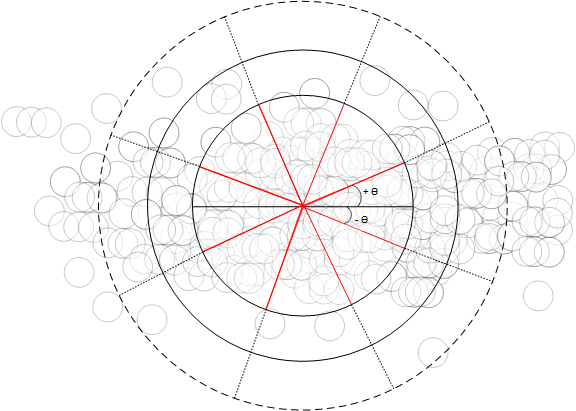
\includegraphics[scale=0.42]{QuantificationSpherique.png}
    \caption{Spheric
     quantizaton}\label{fig:Qantification sph�rique}
\end{figure}


Once this quantization is done, the signature can be constituted by concatenate the values in a vector following a spiral for each value of $\beta$. The histograms obtained for each interval of $\beta$ will be concatenate to obtain the whole signature. 



\begin{figure}[h]
    \center
    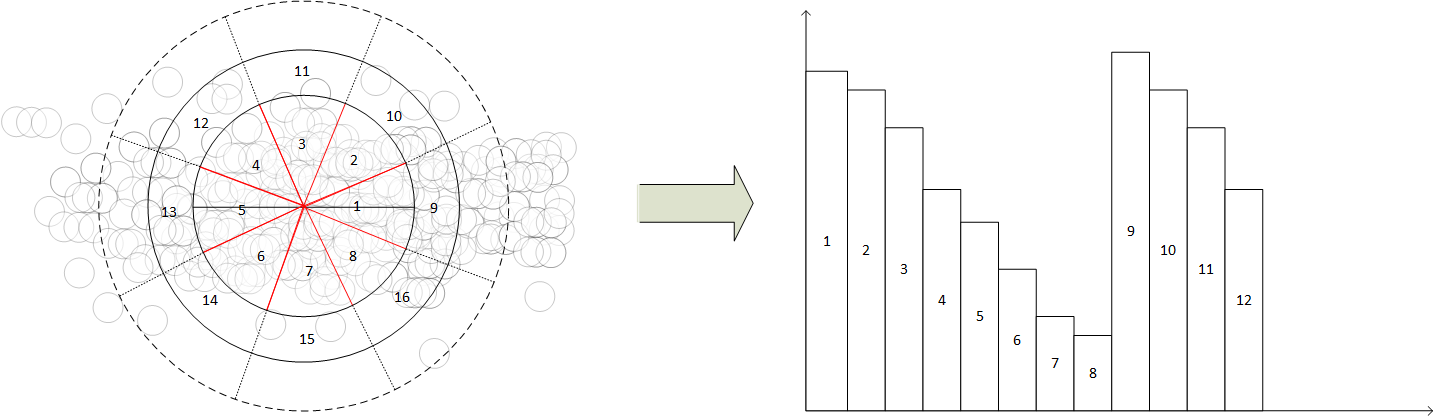
\includegraphics[scale=0.40]{QuantificationSphericToHist.png}
    \caption{Spheric quantizaton to signature}\label{fig:Qantification sph�rique}
\end{figure}


In this way, we obtain one unique vector of 72 values to describe the image.











% ----------------------------------------------------------------
\end{document} 